\documentclass[a4paper, 12pt]{report}

\usepackage[T2A]{fontenc}
\usepackage[utf8]{inputenc}
\usepackage[english,russian]{babel}
\usepackage{amssymb,amsfonts,amsmath,mathtext,cite,enumerate,float}
\usepackage{graphicx}
\usepackage{tabularx}
\usepackage{geometry}

\makeatletter
\renewcommand{\@biblabel}[1]{#1.}
\makeatother

\geometry{left=3cm}
\geometry{right=1cm}
\geometry{top=1cm}
\geometry{bottom=1cm}

\renewcommand{\theenumi}{\arabic{enumi}}
\renewcommand{\labelenumi}{\arabic{enumi}}
\renewcommand{\theenumii}{.\arabic{enumii}}
\renewcommand{\labelenumii}{\arabic{enumi}.\arabic{enumii}.}
\renewcommand{\theenumiii}{.\arabic{enumiii}}
\renewcommand{\labelenumiii}{\arabic{enumi}.\arabic{enumii}.\arabic{enumiii}.}

\graphicspath{{images/}}

\begin{document}
	\section*{Потоки}
	
	Мы нарисовали 2 модели - однопоточный процесс и многопоточный. Необходимо понимать, почему возникла идея потоков. Чтобы это понять надо обратиться к диаграмме состояний процессов.
	
	\subsection*{Три типа событий, переводящие систему в режима ядра}
	
	\begin{itemize}
		\item системные вызовы (они же программные прерывания). Система предоставляет пользователю набор функций - API. Вызвав ее, процесс переходит в редим ядра, чтобы код ядра смог обслужить данные системного вызова
		
		\item исключения - ситуации, связанные с ошибками, связанными с ошибками в коде или ситуациями в системе. Два типа: устранимые (приводят к аварийному завершению процесса (напр деление на нуль), ошибка адресации) и неустранимые (страничные прерывания)
		
		\item аппаратные прерывания - несколько групп (исторически): прерывания от системного таймера, прерывания от устройств ввода/вывода (прерывания от внешних устройств, самые многочисленные), прерывания действий оператора.
	\end{itemize}

	Вернемся к диаграмме состояний процесса:
	
	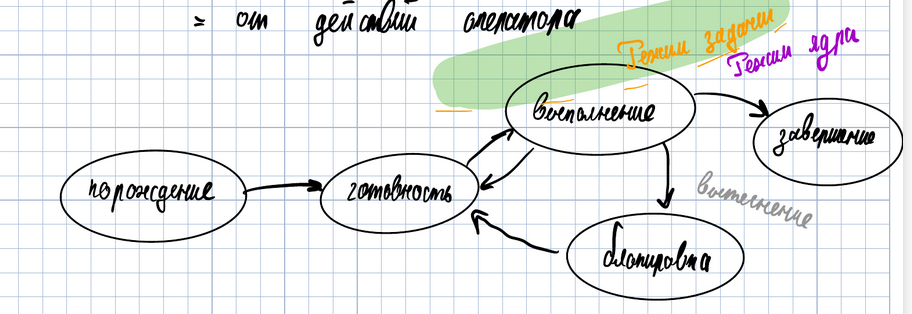
\includegraphics[width=\linewidth]{1}
	
	На этой диаграмме надо отделить действия, выполняемых в режиме пользователя и в режиме ядра.
	
	В UNIX процесс часть времени выполняется в системе (выполняет код программы), часть - в режиме ядра (реентерабельный код ОС).
	
	Нам надо понять, почему возникла идея о потоках. Поток - часть кода, которая может выполняться с другими чатсями кода (причем это непрерывный кусок кода, практически - это задача, которая может выполняться приложением с другими задачами, которые выполняет данное приложение). Хороший пример - Рихтер "Windows для профессионалов", текстовый редактор.
	
	!!! Ни одна система не позволяет процессам напрямую обращаться к устройствам ввода/вывода, поэтому обращение реализовано через системные вызовы.
	
	При запросе дополнительных ресурсов процесс может быть заблокирован. При этом, прерванная работа должна быть возобновлена.
	
	Для того, чтобы продолжить, необходимо сохранить аппаратный контекст (сохранить регистры). Но в современных системах с виртуальной памятью все значительно сложнее. Когда процесс создается, процессу создается адресное пространство (виртуальное), то есть создаются таблицы страниц в современных ОС.
	
	Виртуальное адресное пространстов - это не <<облако>>. Для ОС - это невозможно. В системе создание адресное пространство - это создание соответствующих структур, содержащие адреса соответствующих страниц.
	
	Когда процесс вытесняется (или у него истекает квант проц времени), он переходит из порождения в готовность. Это означает, что кроме аппаратного контекста должен быть сохранен полный контекст (ресурсы, выделенные процессу (в частности - таблицы страниц) + регистры).
	
	Когда, отстояв в очереди, процесс получает процессорное время, контекст восстанавливается.
	
	Сохранение аппаратного контекста часто выполняется. Говорят, что аппаратные прерывания выполняются в контексте процесса. На самом деле, восстановив аппаратный контекст, процесс продолжает работу. Но по истечении кванта, выполняется сохранение полного контекста - затратно для системы, так как задействован не только аппаратный контекст, но и дополнительные системные ресурсы и регистры. Чтобы сократить такие накладные расходы на переключение полного контекста (и из соображений возможности параллельного выполнения частей кода приложения), были введены {\bf потоки}.
	
	Очевидно, что в каких-то приложениях могут выделяться части кода, которые могут выполняться параллельно (где-то нет). Но система не может выполняться разными образами (ветвляться по разным случаям). Поэтому для общности вводятся однопоточные и многопоточные системы.
	
	Потоки разделяют адресное пространство процесса (разделяют код и данные, но стек у каждого потока - свой!). Это явно видно из картинок, которые мы нарисовали.
	
	Цитата: 1.Потоки очень полезны в современном программировании, когда процесс имеет несколько задач при выполнении независимо от других. 2. Это особенно справедливо, когда одна задача может блокироваться, а другие - продолжали выполнение без блокировок. 3. Подтверждение второго - тектовый редактор: фоновый бекграунд-поток может проверять правописание в то время, как другой поток загружает изображение жесткого диска, а четвертый периодически выполняет автоматическое резервное копирование файла, который был отредактирован. (Джефри Ректор (???)).
	
	Достоинства многопоточности:
	\begin{itemize}
		\item отзывчивость (responsiveness) - один поток может обеспечить быструю реакцию, в то время как другие потоки блокированы или медленно выполняют большой объем вычислений; 
		
		\item разделение ресурсов (resource sharing) - по умолчанию, потоки разделяют общий код, данные и другие ресуры, что позволяет нескольким задаам выполняться одновременно в одном адресном пространстве (уточнение: коль скоро потоки разделяют общее адресное пространство, потоки могут использовать одни и те же глобальные переменные, что для процессов требует специальных системных вызовов - средств ядра, потому что адресные пространства процессов  являются защищенными)
		
		\item экономичность (economy) - создание и управление потоками, а именно переключение контекста, является много более быстрым, чем выполнение тех же действий для процессов, потому что при переключениии потоков одного процесса сохраняется только аппаратный контекст.
		
		Можно сказать, что это одна из базовых причин введения многопоточности (расчет на то, что будет переключаться только аппаратный контекст, поскольку параллельные потоки данного процесса выполняются в одном адресном пространстве, поскольку все ресурсы - это ресуры, выделенные процессу, и полный контекст не переключается. Переключение аппаратного контекста поддерживается системно (в винде - popa, pusha))
		
		\item масштабируемость (scalability) - использование мультипроцессорной архитектуры в то время, как однопоточный процесс может выполняться одним процессором (???).
	\end{itemize}
	
	Обсудим следующее. Мы должны понимать, что в системах существует как реальная параллельность (реально параллельно выполняются), так и псевдо-.
	
	\subsection*{Уровень наблюдения}
	
	Рассмотрим систуации:
	
	1. Последовательное выполнение
	
	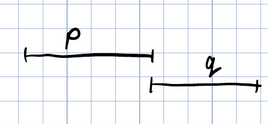
\includegraphics[width=\linewidth]{2}
	
	Характерны для однозадачных систем, когда все ресурсы системы отдаются одному процессу, который выполняется от начала до конца.
	
	2. Если в памяти компьютера одновременно находится большое количество задач/программ, то система имеет возможность переключаться с выполнения одной программы на выполнение другой. Такое переключение выполняется по истечениии кванта.
	
	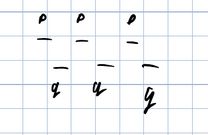
\includegraphics[width=\linewidth]{3}
	
	Это называется {\bf квазипараллельное выполнение}.
	
	Команды каждой программы выполняются последовательно, но пользователю кажется, что программы выполняются параллельно. При этом, параллельные процессы взаимодействуют друг с другом.
	
	3. Реальная параллельность - пересечение выполнения по времени.
	
	
\includegraphics[width=\linewidth]{4}
	
	Упрощенное рассуждение, но оно несет много инфы. На самом деле, время любого процессора квантуется, выполняются и переключение, и вытеснение, и т.д.
	
	Но оказывается, проблема взаимодействия процессов будут общими для систем с реальной параллельностью и квазипараллельным выполнением (???)
	
	Проблемы многопоточности (5 областей, в которых многопроцессорность (multicore) приводит к новым проблемам):
	
	\begin{itemize}
		\item выделение задач для параллельного выполнения (identifying) - необходимо изучать приложения и находить те действия в коде, которые могут выполняться параллельно.
		
		\item сбалансированность - поиск задач для параллельного выполнения, которые обеспечивают равные значения, то есть поток не надо тратиь на тривиальную задачу (<<для Си есть функция swap - на нее не надо тратить поток>>)
		
		\item разделение данных (data splitting) - предотвращать взаимодействие потоков друг с другом.
		
		\item зависимость данных (data dependency) - если одна задача зависит от результатов другой, то задачи должны быть синхронизированы, чтобы обеспечить доступ в нужном порядке (доступ к данным).
		
		\item тестирование и отладка (testing and debugging) - при параллельном выполнении возникают более сложные ситуации, такие как race conditions (<<гонки>>, с точки зрения теории - это доступ параллельных процессов к переменным, данным. Условие возникновения гонок становится сложным для выявления тех мест в коде, [...])
	\end{itemize}
	
	[<<Поздно пить баржоми, когда отвалилась печень>>]
	
	Эти задачи должны быть функционально значимыми (поток проверки орфографии, поток сохранения текстов в файл; все это поддерживает работу текстового редактора)
	
	Потоки, как и процессы параллельные, могут обращаться к одним и тем же данным ({\it разделяемые данные}). Поэтому взаимодействие параллельных процессов требует внимания со стороны разработчика. Требуются глубокие знания параллельного взаимодействия. Необходимо обеспечить монопольный доступ к разделяемым ресурсам. Это обеспечивается методом взаимоисключения.
	
	\subsection*{Типы параллелизма}
	
	Существует два разных пути для распараллеливания нагрузки:
	
	1. Параллельность по датам (data parallelism)
	
	Деление данных между многими ядрами (фактически потоками), которые будут выполнять одинаковые задачи над разными данными (???) [еще пример надо расписать]
	
	2. Параллельность по задачам (по функциям) (task parallelism)
	
	Деление на разные задачи, которые могут параллельно выполняться на разных ядрах.
	
	! Параллельно - не значит одновременно.
	
	Важно понимать, что это разные типы параллелизма.
	
	\subsection*{Модели многопоточности}
	
	Все вокруг этого крутится :)
	
	Существует 2 типа потоков:
	
	1. Уровня пользователя
	
	Программный код делится на потоки, но об этих потоках системе ничего не известно.
	
	
\includegraphics[width=\linewidth]{5}
	
	Имеется библиотека потоков, которая предоставляет все необходимые сервисы. Но для ядра эти потоки не существуют. Для них существует один единственный процесс. Такие билиотеки определены стандартами (в частности - POSIX). Библиотека потоков должна предосталять системе функции для работы над потоками (создание, удаление, переключение контекста, планирование, [что-то еще]).
	
	! Переключение в режим ядра - затратное действие (сохраняется контекст)
	
	Идея библиотеки - уменьшить количество переходов в режим ядра (???)
	
	Все хорошо до тех пор, пока потоки не выполняют системные вызовы. Если какой-то поток запрашивает, например, ввод/вывод, в результате блокируется процесс (система не знает про потоки, которые что-то делают). Более того, в системах разделения времени системы не учитывают работу с пользователем (???) -> по кванту в состояние готовности (???).
	
	Считается, что выигрыш от такого параллелизма условный.
	
	2. Уровня ядра
	
	Потоки, о которых ядру известно.
	
	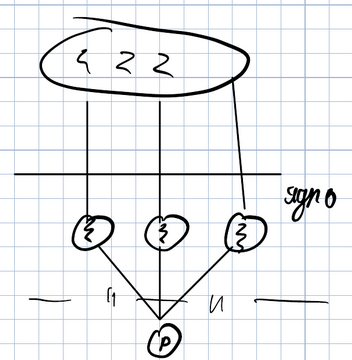
\includegraphics[width=\linewidth]{6}
	
	В системах, в которых мы работаем, реализованы потоки уровня ядра.
	
	Единицей декомпозиции системы остается процесс (он остается владельцем ресурсом). Но потоки ядра выполняются. У них относительный приоитет (относительно базового приоритета процесса системы (???)). При этом на самой первой картинке как раз четко показано, что поток владеет регистрами и стеками.
	
	Так ли все однозначно с выигрышами?
	
	Дело в том, что в системах нет такой дисциплины планирования, которое бы выстраивало бы сначала потоки одного процесса, а потом другого, а потом третьего. Это невозможно, так как потоки выполняются, блокируются, вновь выполняются и т.д. В итоге к процессору стоит смесь потоков, при этом если переключается на поток другого процесса, то сохраняется полный контекст, а внутри одного процесса - аппаратный.
	
	Среднестатистически - время сокращается.
	
	О моделях: все это базируется на том, о чем мы говорили.
	
	1. Модель <<многие к одному>> (many to one)
	
	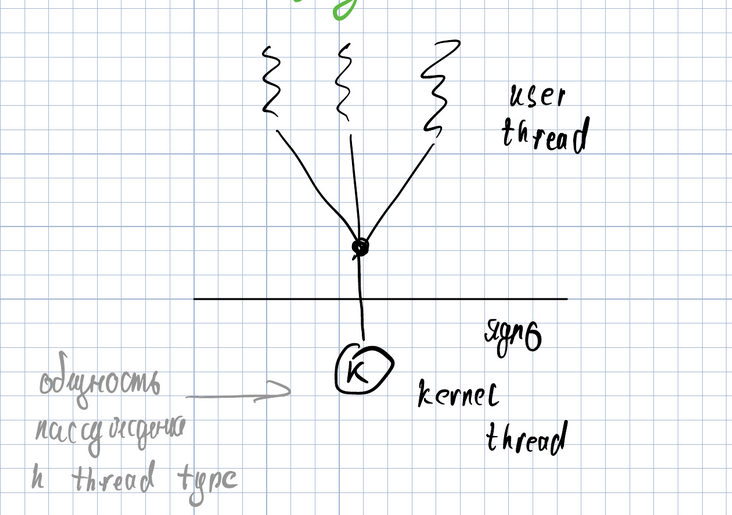
\includegraphics[width=\linewidth]{7}
	
	Управление такой моделью может выполняться с помощью библиотеки потоков уровня пользователя. Пока потоки не запрашивают сервис системы, все прекрасно. Однако если блокирующий системный вызов выполнен потоком, блокируется весь процесс.
	
	Поскольку один поток ядра может выполняться на одном процессоре, модель nк1 не позволяет распараллелить выполнение на несколько процессоров.
	
	Пример: зеленые поток (green thread for Solaris and GNU Portable Threads)
	
	В прошлом эти потоки были реализованы, но некотрые продолжают существовать сегодня.
	
	2. Модель <<один к одному>> (one to one)
	
	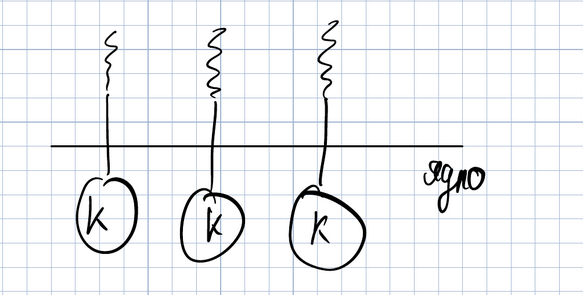
\includegraphics[width=\linewidth]{8}
	
	Потоку приложения соответствует поток ядра, то есть в данной модели создаются отдельные потоки ядра для обработки каждого потока приложения. Соответственно в этой модели нет рассмотренных нами проблем. Если поток запрашивает сервис системы, он будет заблакирован, при этом другие потоки продолжат свое выполнение. Однако считается, что раскладные расхходы достаточно значительны при реализации данно модели, поэтому большинство реализаций ограничивают количество потоков, которые могут быть созданы. Linux и винда реализуют эту модель (правда имеются натяжки).
	
	3. Модель <<многие ко многим>> (many to many)
	
	Продолжим на следующей лекции.
\end{document}
